\documentclass{sig-alternate}

\usepackage{hyperref}

\usepackage{algorithm}
\usepackage{algpseudocode}

\usepackage{booktabs}

\usepackage[draft,nomargin,footnote]{fixme}

\usepackage[usenames,dvipsnames]{xcolor}
\usepackage{tikz}
\usetikzlibrary{positioning, calc}

\usepackage{xspace}
\newcommand{\eg}{\textit{e.g.}\xspace}
\newcommand{\etal}{\textit{et al.}\xspace}
\newcommand{\ie}{\textit{i.e.}\xspace}
\newcommand{\etc}{\textit{etc.}\xspace}
\newcommand{\vs}{\textit{vs.}\xspace}

\graphicspath{{figs/}}

\begin{document}
%
% --- Author Metadata here ---
\conferenceinfo{HRI}{'16 Chrischurch, New Zealand.}
%\CopyrightYear{2007} % Allows default copyright year (20XX) to be over-ridden - IF NEED BE.
%\crdata{0-12345-67-8/90/01}  % Allows default copyright data (0-89791-88-6/97/05) to be over-ridden - IF NEED BE.
% --- End of Author Metadata ---

\title{From Real-time Attention Assessment to ``With-me-ness'' in Human-Robot Interaction}
\author{Fernando Garcia \qquad Séverin Lemaignan \qquad Alexis Jacq \qquad Pierre Dillenbourg\\Computer-Human Interaction in Learning and Instruction Laboratory (CHILI)\\École Polytechnique Fédérale de Lausanne (EPFL)}


\maketitle
\begin{abstract}

Successfully sustaining face-to-face interaction between humans and robots
mandates fine perception of each other attentional focus. This article presents
a novel open-source technique to assess the visual focus of attention (VFoA)
based on accurate, real-time head pose estimation with a single monocular
camera.  Using manual video annotations as ground truth, we show that our system
reaches satisfactory levels of accuracy in a real-world face-to-face interaction
scenario.

We secondly propose to introduce the concept of ``with-me-ness'', borrowed from the
field of {\it Computer-Supported Collaborative Learning}, as an
\emph{in-the-moment} measurement of the quality of interaction. We argue that
this new metric, more specific than the broad concept of engagement, may be well
suited for operational, real-time assessment of an on-going interaction.

\end{abstract}

%% A category with the (minimum) three required fields
%\category{H.4}{Information Systems Applications}{Miscellaneous}
%%A category including the fourth, optional field follows...
%\category{D.2.8}{Software Engineering}{Metrics}[complexity measures, performance measures]

\terms{Experimentation, Human Factors.}

\keywords{Human-Robot Interaction; Social Robotics; Attention Assessment; Engagement; Computer Vision.}

%%%%%%%%%%%%%%%%%%%%%%%%%%%%%%%%%%%%%%%%%%%%%%%%%%%%%%%%%%%%%%%%%%%%%%%%%%%%%%%%%
%%%%%%%%%%%%%%%%%%%%%%%%%%%%%%%%%%%%%%%%%%%%%%%%%%%%%%%%%%%%%%%%%%%%%%%%%%%%%%%%%
%%%%%%%%%%%%%%%%%%%%%%%%%%%%%%%%%%%%%%%%%%%%%%%%%%%%%%%%%%%%%%%%%%%%%%%%%%%%%%%%%

\section{Introduction}

%In the recent years, research is pushing forward in building intelligent systems
%and environments that try to maximize the benefits of cooperation with humans
%based on verbal and non-verbal communication. The interaction between social
%robots and humans entails a broad set of situations, and evidences the need for
%capturing significant backchannel information generated by the user during the
%interaction process. Such information is used to adapt the system to the
%specific user's needs to eventually provide a social or emotional intelligence
%to the agents.
%
%It is indeed not enough to exhibit human-like capabilities in social tasks: a
%robot needs to achieve human-like manners. For instance, several studies showed
%that humans prefer to interact with robots whose task outcome is delayed, shows
%uncertainty or an undesired output \cite{Admoni,Short}. In fact, the ability to
%adapt has been proved to be beneficial in long-term interactions
%\cite{Tielman:2014, Lim:2014}, specifically with children, manifesting a more
%positive attitude over time.

Building capable social agents requires to equip them with a range
of perceptual capabilities: while face and object tracking and
recognition, path planning, speech recognition or task learning are some of the current major research
directions, existing literature tends to evaluate each of these algorithms in
their own metric space, without considering the interaction quality at a global
level: Anzalone~\etal~\cite{anzalone} have recently argued in favor of
such a global evaluation, and they propose to assess these algorithms in term of
their capability to \emph{obtain the desired effect} in a human-robot interaction
context. They correspondingly propose metrics build around the measurement
of \emph{engagement} as indicator of the quality of the experience.

``Engagement'', the cognitive, affective and behavioral state of interaction
with a computer application that ``makes the user want to be
there"~\cite{OBrien:2010}, has actively been studied in a diverse set of
domains. Specifically in robotics, several variables and social signals have been proposed in the
literature to quantify it. A recent review of these is presented in~\cite{ivaldi2015towards}.

%In a learning context, the evaluation of response times in relation with
%correctness has been proposed~\cite{Beck} to provide estimate the user's 
%engagement, with however large inter-subject and environment variability.
%Biometric measurements have also been proposed, like the use the weight
%distribution of the user on a pressure-sensitive
%chair~\cite{Chipman07postureas}.

For instance, \cite{Castellano:2009} proposes to predict children's level of
engagement by integrating in a Bayesian model non-verbal cues (gaze and smiles)
with the current state of the interaction. While they report high level of
accuracy, their approach requires post-hoc video annotations, and is not
applicable to on-line engagement assessment. Similarly,
Baxter~\etal~\cite{baxter2014tracking} posit that the measure of the direction
and timing of gaze in child-robot interactions is a proxy for engagement and
attribution of social agency. However, they also conduct these measures as
post-hoc analyses.  \cite{peters2010investigating} model the user's interest and
engagement with a virtual agent by tracking eye gaze and head direction.
Similarly, \cite{ishii2011combining} estimates the user's engagement with a
conversational agent based on the analysis of gaze patterns.
In~\cite{Rich:2010}, a computational model based on the recognition of
\emph{connection} events such as directed gaze, mutual facial gaze is proposed. Not
relying on gaze, \cite{Sanghvi:2011} focus only on the back or trunk posture as
a determining factor for the assessment. Dinally, a recent study with
social robots in face-to-face scenarios~\cite{anzalone} explores a set of metrics based on
non-verbal cues but they also underline possible limitations in long-term
scenarios.

The variety of these approaches reflects the fact that \emph{engagement} remains
a broad concept, fairly ill-defined and thus difficult to operationalize.
Therefore, instead of introducing ``yet another metric of engagement'', we
propose in this paper to introduce the more specific concept of
``\emph{with-me-ness}'': to what extend the human is ``with me'', the
robot, during the interaction.

We assess this level of ``with-me-ness'' by combining real-time estimation of the
attentional focus of the human with the expected, {\it a priori} focus
requested by the task, as estimated by the robot.

This article is organized in three sections: we first present a novel
method for on-line estimation of the focus of attention based on fast 6D head
pose estimation. We then propose to validate this approach with 
a real-world field experiment with children. We finally show how to compute
``with-me-ness'' over the course of the interaction to provide a new \emph{in-the-moment} measurement of
the quality of interaction, and compare levels computed by the robot with a
ground truth based on manual post-hoc annotations.

%\paragraph{Motivation: Impact on Learning}
%
%Education and learning environments are interesting application fields for
%research on attention assessment, since sustaining children's engagement over
%time is a key variable to ensure effective learning (see for
%instance~\cite{Umbach}), and they indeed motivate this research. In fact, the
%use of robots in education comes with the potential to engage the child in
%meta-cognition through the learning by teaching paradigm, wherein a student
%takes the role of a teacher and experiences stronger educational benefits as a
%result (such as in \cite{Palinscar1984}).
%
%While~\cite{zhao2012learning} recommends the development of a teachable agent
%that is actively, rather than passively, engaged in the learning by teaching
%interaction, the increased learning gain results attained
%in~\cite{okita2006observation} were done so even with the pupil being taught
%having been instructed to not contribute much information. This suggests that it
%may not be necessary, from a learning by teaching point of view, for the
%teachable agent to participate actively in the interaction to incite educational
%benefits. However, from an engagement point of view, this may not necessarily be
%true.
%
%The goal of this research is therefore to \textbf{evaluate the quality of an
%interaction} using the \textbf{visual focus of attention as an engagement
%indicator}. We validate our approach with field experiments conducted in the
%educational context of the CoWriter project~\cite{Hood:2015}, where our
%technique, being based on a regular, low-end RGB camera, avoids the use of
%otherwise typically invasive technologies such as eyetrackers, that would
%negatively impact the natural of the interaction.


%%%%%%%%%%%%%%%%%%%%%%%%%%%%%%%%%%%%%%%%%%%%%%%%%%%%%%%%%%%%%%%%%%%%%%%%%%%%%%%%%
%%%%%%%%%%%%%%%%%%%%%%%%%%%%%%%%%%%%%%%%%%%%%%%%%%%%%%%%%%%%%%%%%%%%%%%%%%%%%%%%%
%%%%%%%%%%%%%%%%%%%%%%%%%%%%%%%%%%%%%%%%%%%%%%%%%%%%%%%%%%%%%%%%%%%%%%%%%%%%%%%%%

\section{Visual Attention Assessment}
\label{sec:vfoa}

\subsection{Related Work}

The relation between one's focus of attention and what he/she is looking at has
long been established~\cite{yarbus1967eye,barber1976perception}, and more
specifically, the existing relationship between gaze and attention during social
interaction, and the related gaze patterns, has been part of classic textbooks
like~\cite{argyle1969social} since decades. As such, there is little doubt that
measuring the direction of gaze is a useful proxy to estimate the (visual) focus
of attention of a social agent, and indeed this is one of the basic tool used in
social psychology.

Estimating attention using gaze is not new to robotics either. A
recent survey by Ruhland~\etal~\cite{ruhland2015review} presents in a synthetic
way eye gaze research in HCI and social robotics. It remains however an active field of research, as illustrated by
several recent publications~\cite{baxter2014tracking,anzalone,kennedy2015head}:
performing such a measure on a robot, in real-time, and in ecologically
valid environments (which rules out bulky or invasive apparatus like
eye-trackers, or techniques requiring fine calibration and/or static
interactions) remains a challenge in HRI.

Looking at techniques that both operate on-line and have been deployed in field
experiments, one finds that most approaches rely on head pose estimation alone
(no eye gaze tracking) and are generally based on depth sensors (RGB-D) .
Fanelli~\etal provides a overview of these approaches in~\cite{fanelli2012real},
and recent examples include~\cite{baxter2014tracking, anzalone}.

Approaches based on monocular 2D vision have been explored as
well~\cite{peters2010investigating}, with however limited robustness to
occlusions or lightning conditions, and over-reliance on tracking to maintain
real-time performances.  Our work relies on recent advances on template-based
face alignment~\cite{kazemi2014one} that allows fast (in the order of a few
milliseconds) facial features extraction on 2D images, combined with 3D model
fitting, to obtain a fast, robust and stable 6D head pose estimate, that we
successfully deployed in field experiments involving child-robot interactions.

We derive the field of attention from the head pose: this is supported by
previous work, like~\cite{stiefelhagen2002tracking} that shows that the head orientation's contribution in
overall gaze direction is 68.9\%, which further translates into a 88.7\%
accuracy in estimating the focus of attention from head pose only in a
particular meeting scenario (using eye and head tracking).

While previous preliminary research in HRI seemed on the contrary to indicate that deriving
attentional focus from head pose alone would not be accurate
enough~\cite{kennedy2015head}, we found in our case acceptable levels of
agreement between the robot observations and manual post-hoc annotations, as
detailled hereafter.

\subsection{Head Pose Estimation}

As explained, we derive the visual field of attention from the head pose. Our
technique only involves a single monocular RGB camera used for facial
feature extraction, and a static simplified 3D mesh of a human head.
68 facial features are extracted using a fast
template-based face alignment algorithm by Kazemi and
Sullivan~\cite{kazemi2014one}, as implemented in the open-source {\tt dlib}
library~\cite{dlib09}.  Eight of these features are
then matched to their 3D counterparts (Figure~\ref{head_pose}) and we rely on an iterative $PnP$ algorithm
(OpenCV's implementation) to compute the translation and rotation of the head
with respect to the camera frame. With this approach, knowing the intrinsic
parameters of the camera (calibrated camera) is required for an accurate
estimation of the absolute 3D localization of the head.

Besides being fast, the face alignment algorithm has been found to perform well
in terms of robustness, including in a range of difficult situations
(occlusions, large head rotations) as encountered in field experiments.
Figure~\ref{head_pose_real_world} shows a selection of such difficult scenes with
one child.

\begin{figure}[t]
    \centering
    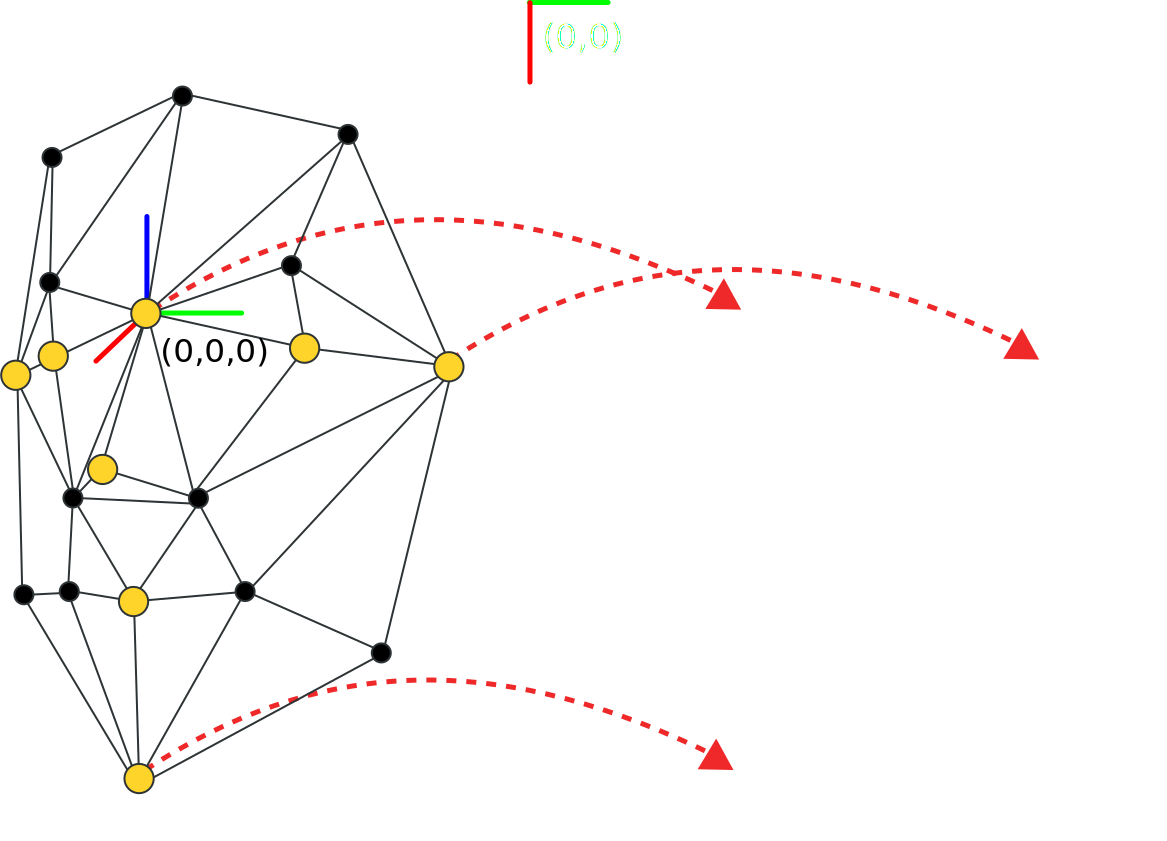
\includegraphics[width=0.9\linewidth]{head_pose}
    \caption{The 6D head pose is estimated by fitting a 3D model of an
        adult head (left) onto the detected 2D features of the face (right). We
        rely on an iterative $PnP$ algorithm, using 8 correspondence pairs
        (three are depicted: the sellion -- the nasal depression --, the left
        tragion and the menton). The 3D origin of the head is set at the sellion.}

    \label{head_pose}
\end{figure}

\begin{figure}[t]
    \centering
    
\includegraphics[width=\linewidth]{head_pose_real_world}
    \caption{Head pose results on images captured during a field experiment.
    Detection of face features (and therefore, estimation of the pose) is robust
    to significant occlusions and face rotations.}
    \label{head_pose_real_world}
\end{figure}

\subsection{Field \& Focus of Attention}

\begin{figure}
    \centering
    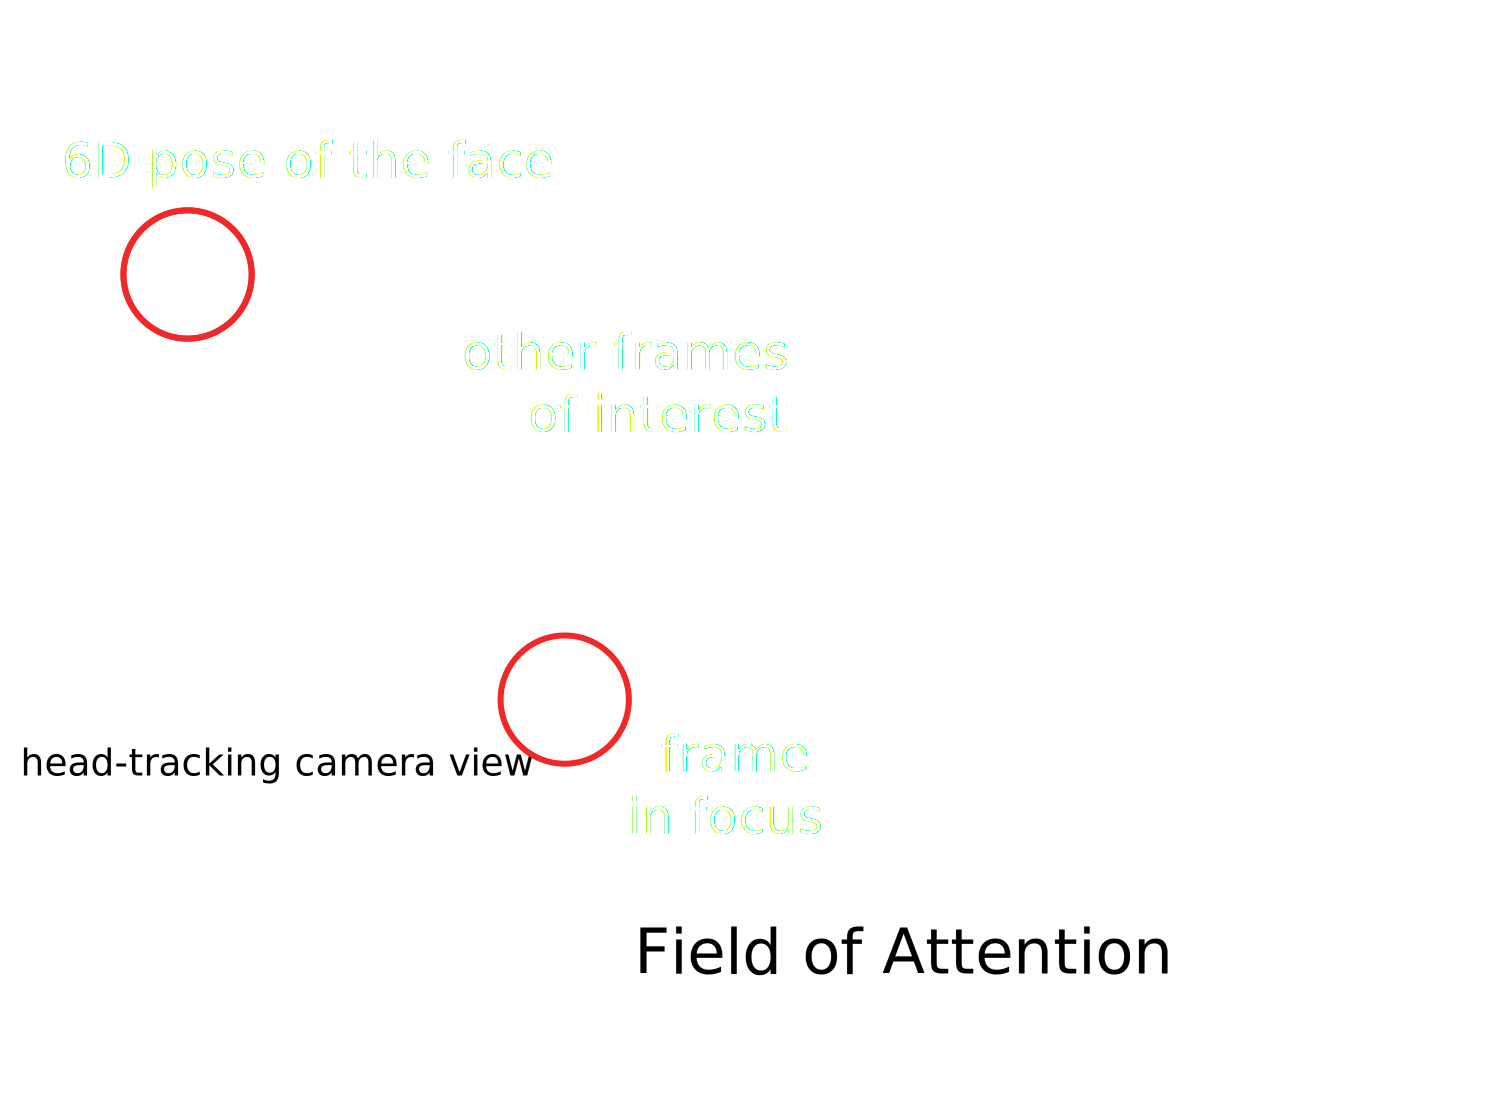
\includegraphics[width=0.9\columnwidth]{field_of_attention}
    \caption{\small The visual field of attention is approximated to a
        40$\degree$ cone, spanning from the head's sellion. The objects whose 3D
    pose intersect with this cone are considered \emph{in focus}.}
    \label{fig:vfoa}
\end{figure}

We model the field of attention as the central region of the field of view.  The
field of view itself is approximated to a cone spanned from the nasal depression
(sellion) of the human face. Different dimensions for the human field of view
can be found in the litterature: Holmqvist~\cite{holmqvist2011eye} models it
with an horizontal aperture of $ \pm 40\degree $ and a vertical aperture of $
\pm 25\degree $, while Spector~\cite{walker1980clinical} for instance suggests
$60\degree$ up, $75\degree$ down, $60\degree$ inwards (towards the nose) and
$95\degree$ outwards.  Previous work on visual perspective taking for social
robotics~\cite{sisbot2011situation} model the field of attention as a cone of
$30\degree$. We retained in this work a slightly wider aperture of $40\degree$.

We then approximate the visual \emph{focus} of attention (VFoA) of the human to the
objects which lay inside this field of attention (Figure~\ref{fig:vfoa}). At a
given time, more than one object can therefore be \emph{in focus}.

Our implementation has two limitations: objects are approximated to points
(their origin), and we do not
check actual visibility: one object could be hidden by another, it would still
be considered as in focus. We did not address these limitations since our
experimental setup (involving relatively small objects with no occlusions) did
not mandate it. Techniques for more accurate assessment of the visual
perspective of the human peer can be found in~\cite{sisbot2011situation} for instance.

Within these limitations, computing if object $A(x_A,y_A,z_A)$ is in the field
of attention of the human requires first to transform the coordinates
$A(X_A,Y_A,Z_A)$ into the frame of the face, and then to verify the following
simple inequality (with $fov$ the aperture, and assuming that the main axis
$\vec{x}$ of the field of attention points forward):

\begin{align}
    \sqrt{Y_A^2 + Z_A^2} < tan\left(\frac{fov}{2}\right) \cdot X_A
\label{eq:fov}
\end{align}

Our approach assumes that the pose of the objects of interest are available to
the system: as described in section~\ref{sec:system}, our implementation relies
on the ROS {\sc tf} framework to manage and make available to all software
modules the list of poses of existing objects (represented as {\it frames}), and
dedicated perception modules are in charged of publishing up-to-date
informations regarding the location of the objects of interest (the so-called
\emph{situation assessment}). Due to the nature of the experiment, most of the
points of interest considered for the experimental validation presented
hereafter are static with respect to the robot, thus simplifying the scene
perception.

%%%%%%%%%%%%%%%%%%%%%%%%%%%%%%%%%%%%%%%%%%%%%%%%%%%%%%%%%%%%%%%%%%%%%%%%%%%%%%%%%
%%%%%%%%%%%%%%%%%%%%%%%%%%%%%%%%%%%%%%%%%%%%%%%%%%%%%%%%%%%%%%%%%%%%%%%%%%%%%%%%%
%%%%%%%%%%%%%%%%%%%%%%%%%%%%%%%%%%%%%%%%%%%%%%%%%%%%%%%%%%%%%%%%%%%%%%%%%%%%%%%%%

\section{Experimental Validation}
\label{sec:expe}

As presented above, we use the 6D head pose as an approximation of the
actual gaze direction, and we further approximate from here the participant's field of
attention. The assumption that such an double approximation of the field of attention
allows to derive the actual focus of attention needs to validated experimentally.
Our proposed experiment involves child-robot
interactions in the context of handwriting remediation.
This section details the experimental procedure and presents our results.


\subsection{Experimental Procedure}

The experiment, part of the CoWriter project~\cite{Hood:2015}, involves a robot
which tries to engage a child in handwriting tasks using a \emph{learning by teaching}
paradigm (\ie the child is the teacher, and he/she attempts to improve the
robot's handwriting). A tactile tablet is used as writing support.

\begin{figure}[h!]
    \centering
    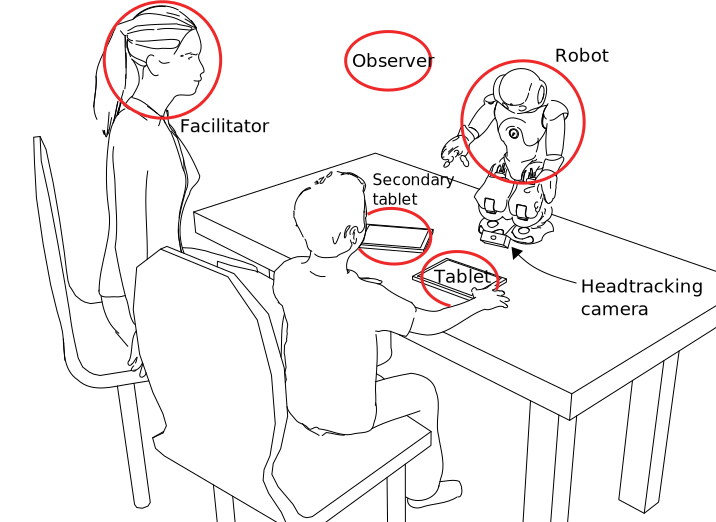
\includegraphics[width=0.8\columnwidth]{experimental_setup}
    \caption{\small \textbf{Experimental setup}: face-to-face interaction with a {\sc
            nao} robot. The robot writes on the tactile tablet, the child then
            corrects the robot by directly overwriting the words on the tablet
            with a stylus. The facilitator remains next to the child to guide the work. 
            The secondary tablet allows the child to tell the robot what to
            write. The areas of interest -- corresponding to potential target of
            attention -- are circled in red with their name.}
    \label{fig:setup}
\end{figure}


Figures~\ref{fig:setup} and~\ref{fig:realSetup} illustrate the experimental setup: a face-to-face
child-robot interaction with an (autonomous) Aldebran's {\sc nao} robot, in
presence of a facilitator (one of the researchers).

\begin{figure}[h!]
    \centering
    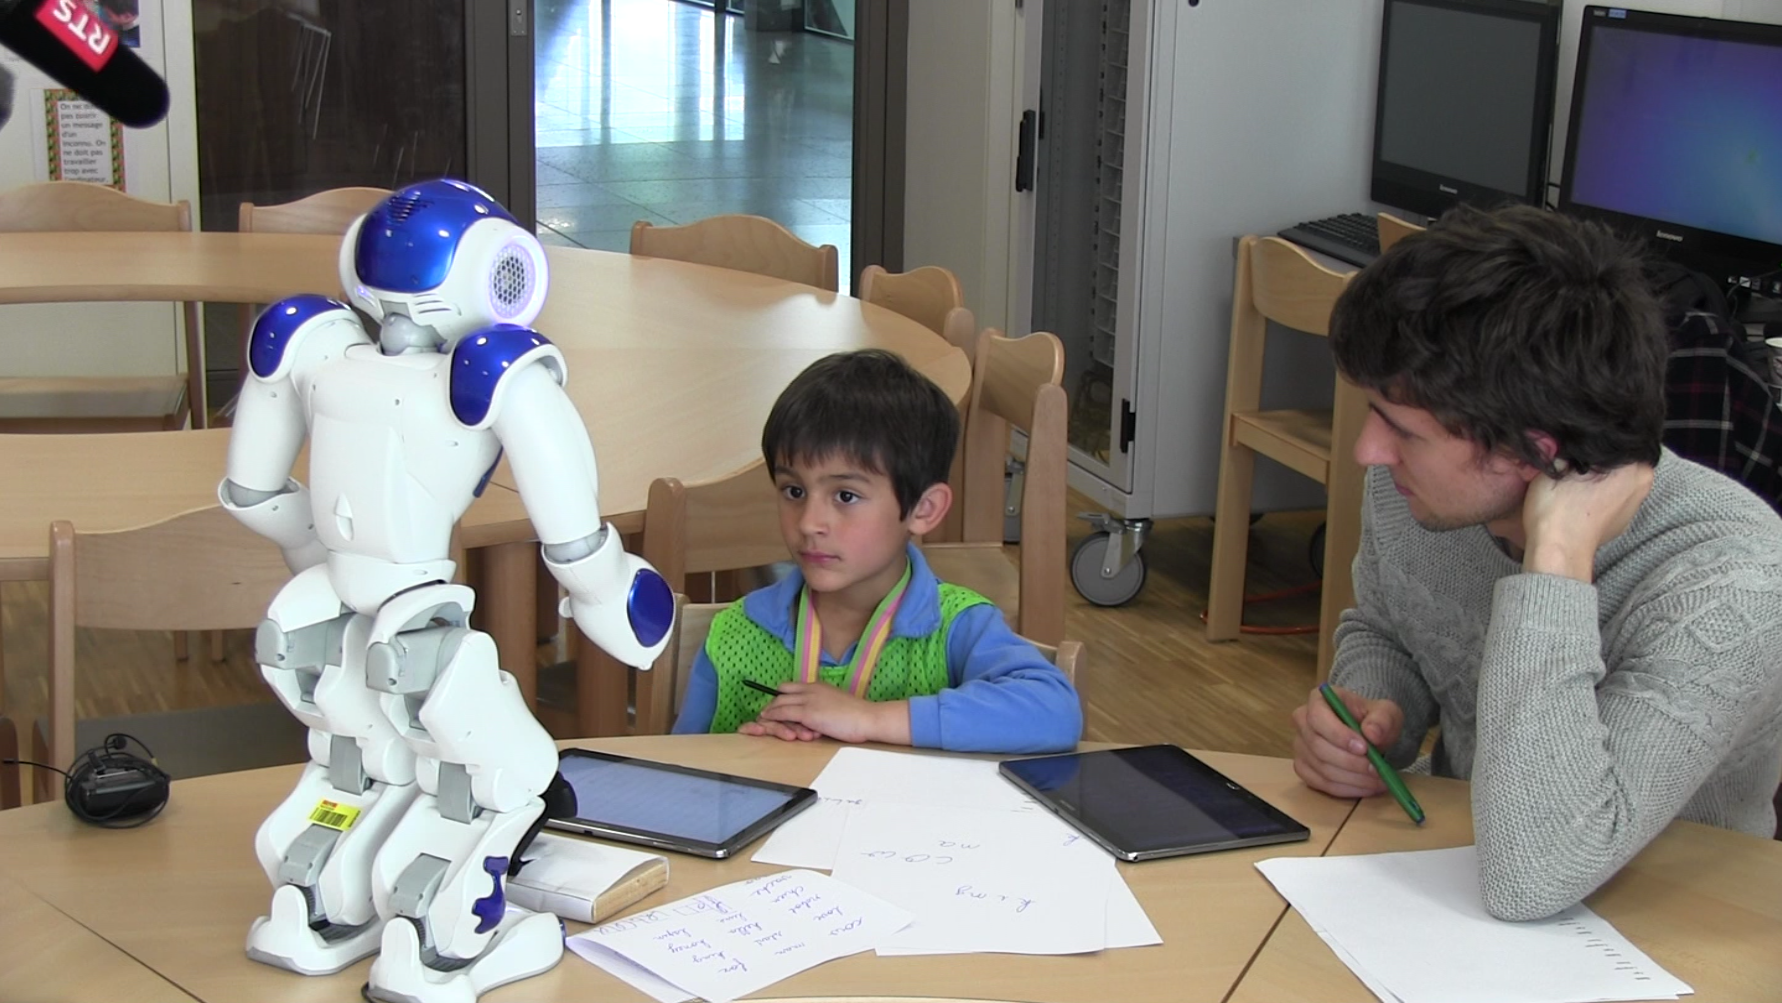
\includegraphics[width=1\columnwidth]{realSetup}
    \caption{\small Picture of the interaction with one of the children.}
    \label{fig:realSetup}
\end{figure}

The subjects were typically located 50 cm away from the robot with the primary
(writing) tablet in front and the secondary one 30 cm to the left of the first
one.  The facilitator was located about 60 cm to the left of the subject.
Finally, two observers were located further away from the interaction field.
Figure~\ref{fig:setup} indicates accordingly the location of main areas of
interest (the two tablets, the robot, the facilitator and the observers).


The dependent variable is the measurement of the participants' VFoA, assessed in
terms of what are the attentional targets of the child over time. The face of the child
is acquired through a fixed webcam (Logitech {\sf c920}), placed on the table
(see Figure~\ref{fig:setup}), and the attentional targets are then computed as
presented in section~\ref{sec:vfoa}.

%An RGB camera has been used to acquire images of 640x480 pixels at 25 fps. The
%camera was located at 5 cm from the center of nao's feet and its holder was tied
%to a wood base for stability purposes. Thus, the camera's objective was 9 cm
%above and $ 40\degree $ inclination with respect to the surface of the table to
%maximize the detection during the writing time. However, nao's camera could have
%been used, always considering the \textit{tf} frame matrix update according to
%the head orientation.

\subsection{Experimental Procedure}

Six children (ages 5 to 6, 3 boys, 3 girls) were enrolled for this study.
The study took place at school, in a separate room (the computer
lab). The participants were chosen by the teacher, and would come one after the
other to interact with the robot (duration: $M=19.6$ min, $SD=1.58$).

The interaction is organized in rounds of writing: during a typical round, the
child requests the robot to write something (a single letter, a number or a full
word), and presents a tactile tablet (equipped with a custom writing
application) to the robot; the robot writes on the tablet by mimicking the
writing gesture (but without actually physically touching the tablet); the child
then pull back the tablet, corrects the robot's attempt by writing him/herself
on top or next to the robot's writing, and ``send'' his/her demonstration to the
robot by pressing a small button on the tablet. The robot learns from this
demonstration and tries again. The child continues the turn-taking until he/she
decides to train the robot on another word. In total, the children performed in
average 12.16 ($SD=2.61$) rounds of writing (complete details on the rationale
and implementation of this experiment can be found in~\cite{Hood:2015}).


Besides, once per interaction, the robot interrupts the handwriting task to
propose to tell a story (taking about 2 min), and the turn-based
hand-writing task continues afterwards. The intended purpose of the
story-telling episode is to locally trigger a different set of attention behaviors.


\subsection{System Implementation}

\label{sec:system}

\begin{figure}[h!]
    \centering

\resizebox{0.9\linewidth}{!}{%

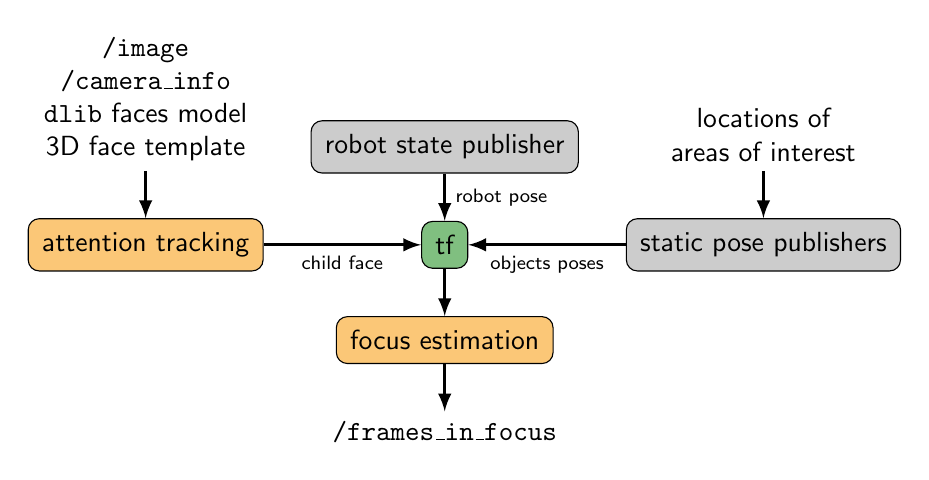
\begin{tikzpicture}[
    >=latex,
    node distance=2cm,
    every edge/.style={draw, very thick},
    redarrow/.style={fill=Red, draw=Red},
    greenarrow/.style={fill=GreenYellow, draw=GreenYellow},
    yellowarrow/.style={fill=BurntOrange, draw=BurntOrange},
    cmpt/.style={draw, align=center, rounded corners, inner sep=5pt, font=\sf, fill=black!20},
    label/.style={midway, align=left, font=\scriptsize\sf, fill=white, above,opacity=0,text opacity=1}]

%    \node at (0,0)[cmpt, fill=Cyan!50, text width=2.7cm] (tactile) {tactile interaction \\ manager};

    \node at (0,0) [cmpt, fill=Green!50] (tf) {tf};
    \node [cmpt, fill=YellowOrange!50, left=of tf] (attention) {attention tracking};
    \node [above=0.6cm of attention, text width=2.7cm,align=center] (input) {\tt /image \\ /camera\_info \\ dlib {\sf faces model} \\ {\sf 3D face template}};
    \node [cmpt, right=of tf] (static) {static pose publishers};
    \node [above=0.6cm of static, text width=2.7cm,align=center] (staticposes) {\sf locations of \\areas of interest};
    \node [cmpt, above=0.6cm of tf] (pose) {robot state publisher};
    \node [cmpt, fill=YellowOrange!50, below=0.6cm of tf] (focus) {focus estimation};
    \node [below=0.6cm of focus] (output) {\tt /frames\_in\_focus};

    \path (staticposes) edge [->] (static);
    \path (static) edge [->] node[label,below] {objects poses} (tf);
    \path (input) edge [->] (attention);
    \path (attention) edge [->] node[label,below] {child face} (tf);
    \path (pose) edge [->] node[label,right] {robot pose} (tf);
    \path (tf) edge [->]  (focus);
    \path (focus) edge [->]  (output);

\end{tikzpicture}
}

    \caption{\small ROS nodes involved in the VFoA estimation (yellow nodes were developed for this work).}
    \label{fig:system}
\end{figure}

The experiment was carried with an Aldebaran's {\sc nao} robot, using ROS as a
middleware to build the attention estimation pipeline (Figure~\ref{fig:system}).
Head pose estimation, presented in section~\ref{sec:vfoa}, builds on the {\tt
dlib} and OpenCV libraries; the pose transformations are handled by the ROS {\sc
tf} library. The same {\sc tf} library is used to represent as individual frames
the possible point of interests: an object is considered to be in focus when its
frame lays within the field of attention of the participant
(Figure~\ref{fig:vfoa}).  The implementation is open-source and available at
\url{https://github.com/chili-epfl/attention-tracker}.

The implementation of the hand-writing activity itself has been presented by
Hood~\etal in~\cite{Hood:2015}.

\subsection{Data Collection \& Analysis}

Successful detections of the head, and, when detected, the attentional targets of
the children as estimated by the robot, were logged during the experiment (in
total, $6\times19.6=117.6$ min of interaction). The only post-processing
consisted in filtering out gaze shifts (short episodes -- below 500ms -- between
two attentional targets).

Besides, we video-recorded the interactions, and performed a {\it post-hoc}
manual coding of the focus of attention by two annotators (Cronbach's
$\alpha=.89$)\fixme{did the 2nd annotator annotated the 6 whole interactions?}.
The manual coding forms our attentional \emph{ground-truth}.

To assess the accuracy of the attention estimation by the robot, we computed
over time (excluding the periods when the head is not detected) the
overlap between the ground-truth and the robot's estimate and the
inter-judge agreement (Cronbach's $\alpha$).
%and the cosine similarity
%matrix.

%The Cronbach's $\alpha$ can be defined as an average of the correlations between 
%the items or values at the same time step \textit{t}. Therefore, results can vary 
%significantly if both sets of values are time shifted. However,
%the cosine similarity becomes a useful measurement in this case as it accounts 
%for temporal delays. Specifically, the ground-truth values acquired though human 
%annotations may not match the measurements of the focuses of attention computed 
%by the robot at the exactly same time step \textit{t} even though the correspondent
%curves may look very similar in shape.

\subsection{Results}

\begin{table*}[ht!]
    \centering
    \caption{\textbf{Attention tracking accuracy}. \emph{Head pose
    tracking} is the percentage of total time of successful detection of the
    head pose; \emph{Agreement} is the percentage of matching time
    between manually annotated focus of attention (ground-truth) and robot's
    computed focus of attention. Total duration: 117.6 min.}

    \begin{tabular}{p{5.5cm}cccccccc}
        \toprule
        {\bf Subject} & 1 & 2 & 3 & 4 & 5 & 6 & {\bf M} & {\it SD} \\
        \midrule
        {\bf Head pose tracking} (\%) & 88.2 & 83.5 & 90.5 & 83.1 & 87.9 & 85.0 & {\bf 86.4} & {\it 3.0} \\ 
        \midrule
        {\bf Agreement} (\%) & 58.9 & 67.1 & 79.2 & 48.3 & 65 & 77.1 & {\bf 65.9} & {\it 11.5}\\
        {\bf Cohen's $\kappa$} & 0.48 & 0.56 & 0.68 & 0.26 & 0.47 & 0.68 & {\bf 0.52} & {\it 0.16}\\
        %{\bf Cosine affinity} & 0.73 & 0.82 & 0.87 & 0.73 & 0.77 & 0.89 & {\bf 0.8} & {\it 0.07} \\
        \bottomrule
    \end{tabular}
    \label{tab:results}
\end{table*}

The main results are reported in Table~\ref{tab:results}
%and Figure~\ref{fig:cosinematrix} (cosine similarity matrix);
Figure~\ref{fig:realExpected} further gives a concrete picture of the
ground-truth \vs computed attentional targets for subject 4 (the subject with
the \emph{least} successful tracking).

%
%\begin{figure}[th!]
%    \centering
%    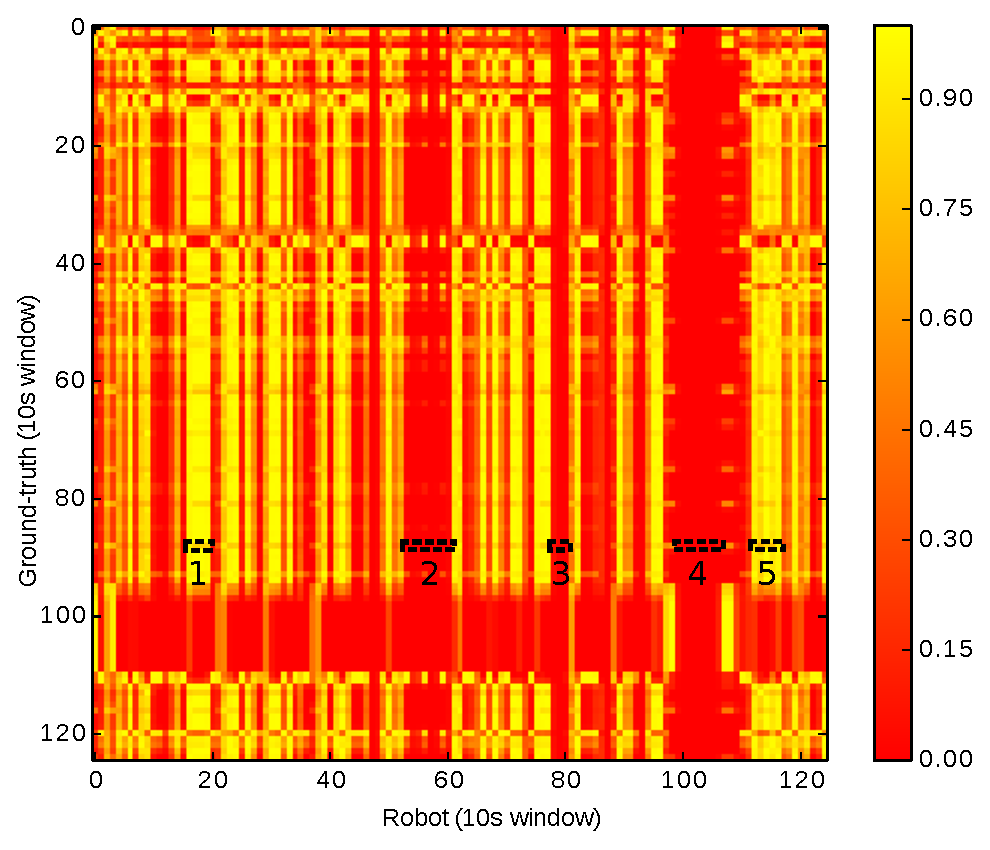
\includegraphics[width=0.7\columnwidth]{bitmap}
%    \caption{\small Cosine similarity matrix between ground-truth and robot-measured VFoA
%    using a 10 sec. window size. The correspondent numbers are shown
%    in figure \ref{fig:realCaptured}.}
%    \label{fig:cosinematrix}
%\end{figure}

\begin{figure*}[ht!]
    \centering
    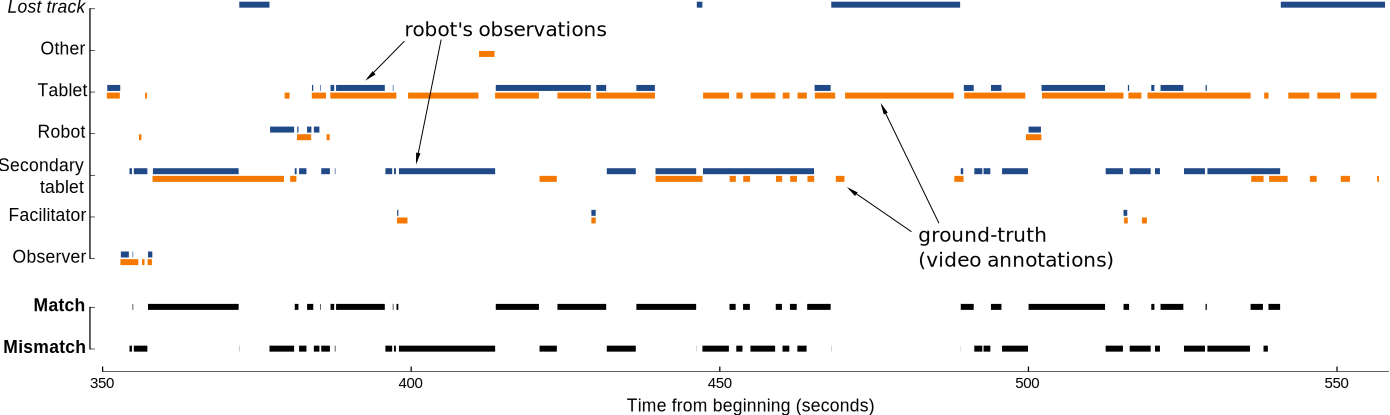
\includegraphics[width=\linewidth]{matches-excerpt}
    \caption{\small \textbf{Comparison of computed focus of attention \vs ground
        truth} during a face-to-face child-robot interaction (subject 4
        in table~\ref{tab:results}, 3.5min-long excerpt).
        In blue (top lines), the focus of attention as computed by the robot;
        in orange (bottom lines), the focus of attention as manually annotated
        (ground-truth). Periods where the head is lost are marked with dashed
        vertical lines. The bottom graph shows agreement between both (whenever
        the head is detected).}

    \label{fig:realExpected}
    
    % Maybe we should add the expected VFoA
\end{figure*}


During the whole interaction, the head pose of the children was satisfactorily
and consistently tracked (86\% of the time in average, $SD=3.0$). While this
high score is expected for a face-to-face interaction with a static head-tracking camera
(meaning that the child head would remain in the field of view of the camera
most of the time), this is still comforting in terms of suitability of our
approach for head pose estimation with children in field experiments of this
kind. Expectedly, the primary causes of lost head pose were occlusions with the
hands (similar to the middle-bottom picture in
Figure~\ref{head_pose_real_world}), close proximity with the tablet while
writing, and gaze directed to the facilitator (who was sitting directly on the left of
the child, Figure~\ref{fig:realSetup}).

In terms of attention tracking, Cohen's $\kappa$ values are between 0.47 and
0.68 with one subject resulting in significantly worst tracking, at 0.26. While
the interpretation of Cohen's $\kappa$ is subject to discussions (the number of
the coded values -- in our case 6 -- and the distribution probability of values
-- in our case, values are \emph{not} equiprobable -- are factors impacting
$\kappa$ independently of the level of agreement), the levels of agreement are
\emph{moderate} to \emph{substantial}, with one subject only
showing \emph{fair} agreement~\cite{landis1977measurement}. Further analysis of
the videos shows that the child with the lowest level of agreement is especially
calm and would rely more on the eyes to direct his gaze than the other children,
thus leading to a less accurate estimation of its focus of attention.

%\subsubsection{Focus of attention distribution}
%
%Additional information of the head pose can be obtained for the evaluation of
%the VFoA distribution. Figure \ref{fig:heatmap} shows the most salient focuses
%of attention where the peaks are located. These peaks are mainly projected
%between the triangle composed by the robot, the writing tablet and the selection
%tablet using an unsupervised K-means clustering method reveals, considering the
%observers as negligible VFoA.
%
%% Workaround to do subfigure since the packege looks not to work
%\begin{figure}[th!]
%  \centering
%  \begin{tabular}{@{}c@{}}
%    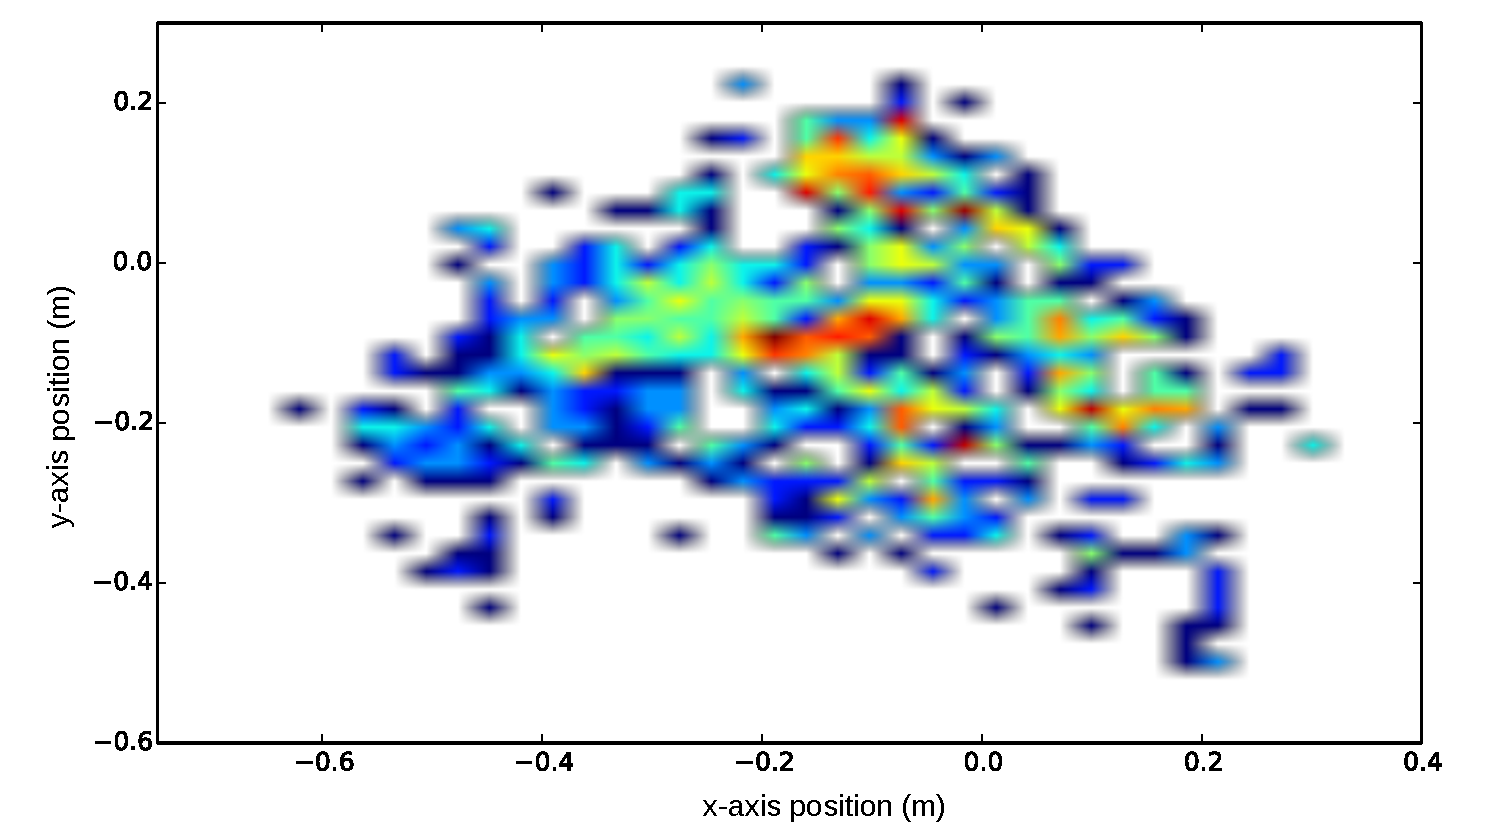
\includegraphics[width=.7\linewidth,height=100pt]{heatmap} \\
%    \small (a)  2D histogram.
%  \end{tabular}
%
%  \vspace{\floatsep}
%
%  \begin{tabular}{@{}c@{}}
%    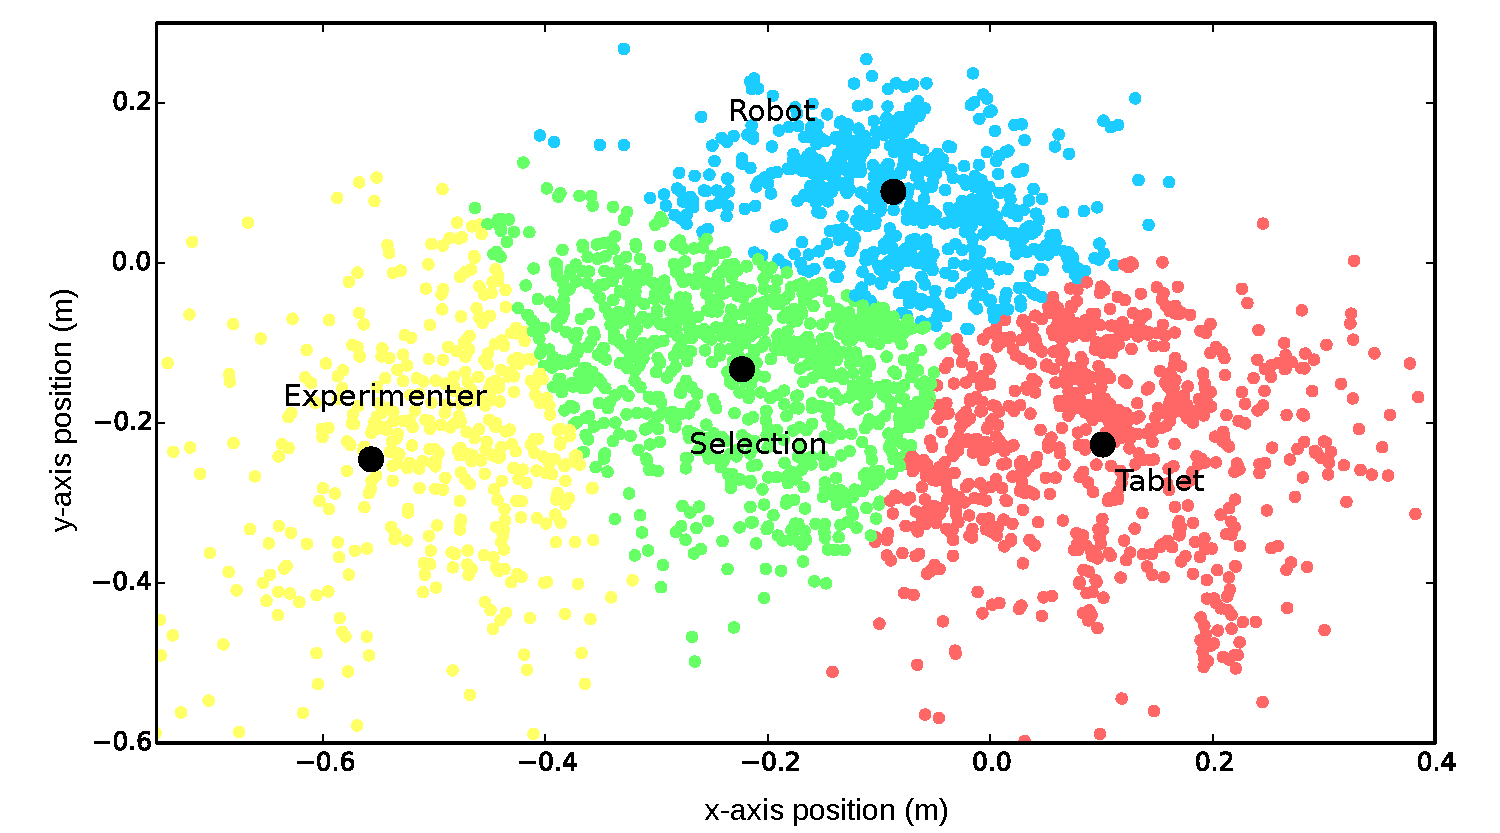
\includegraphics[width=.7\linewidth,height=100pt]{kmeans} \\
%    \small (b) K-means clustering.
%  \end{tabular}
%
%  \caption{ \small Subject 4 head movements. (head yaw on x-axis, pitch on y-axis).}
%  \label{fig:heatmap}
%\end{figure}



%%%%%%%%%%%%%%%%%%%%%%%%%%%%%%%%%%%%%%%%%%%%%%%%%%%%%%%%%%%%%%%%%%%%%%%%%%%%%%%%%
%%%%%%%%%%%%%%%%%%%%%%%%%%%%%%%%%%%%%%%%%%%%%%%%%%%%%%%%%%%%%%%%%%%%%%%%%%%%%%%%%
%%%%%%%%%%%%%%%%%%%%%%%%%%%%%%%%%%%%%%%%%%%%%%%%%%%%%%%%%%%%%%%%%%%%%%%%%%%%%%%%%

\section{With-me-ness}

\subsection{Concept \& Calculation}

The concept of \emph{with-me-ness} has been introduced in the field of
\emph{Computer Supported Collaborative Learning} (CSCL) by Sharma~\etal
in~\cite{sharma2014me}. Sharma~\etal introduce this concept in an attempt to
answer a recurrent teacher's question: {\it ``how much are the students with
me?''}. They distinguish what they call \emph{perceptual with-me-ness} (the
student follows what the teacher refers to with deictic gestures) from
\emph{conceptual with-me-ness} (the student follows what the teacher refers to
verbally), and they show in an eye-tracking study that \emph{conceptual
with-me-ness} in particular correlates with better learning performance. This
also relates to the concept of gaze cross-recurrence that has been shown to
reflect the quality of the interaction~\cite{jermann2012effects} in
collaborative learning tasks.

Sharma~\etal simply define \emph{conceptual with-me-ness} as the normalized
percentage of time during which the student's gaze overlapped the areas of
teaching slides currently referred to by the teacher.
In order to apply it to human-robot interactions, we propose to extend this
concept, and to define \emph{conceptual with-me-ness} as the normalized
ratio of time that the human interactant focuses its attention on the
attentional target expected by the robot for the current task (or sub-task).


\begin{algorithm}[h!]
    \centering

    \begin{algorithmic}[1]
    \Procedure{Compute With-me-ness} {}
    \State $d_w, d_e \gets 0$
    \State $t \gets t_{start}$
    \Repeat
    \If{$task(t) \neq$ nil \textbf{and} \par
    \hskip\algorithmicindent$F(task(t)) \neq \varnothing$ \textbf{and} \par
    \hskip\algorithmicindent $f(t) \neq$ nil } \label{algline:skiplosttrack}
    \If{$f(t) \in F(task(t))$}
            \State $d_w \gets d_w + \delta_t$
        \EndIf
        \State $d_e \gets d_e + \delta_t$
    \EndIf
    \State $t \gets t + \delta_t$
    \Until{$t = t_{end}$}

    \State $\mathcal{W}_{[start, end]} \gets \frac{d_w}{d_e}$
    \State \Return $\mathcal{W}_{[start, end]}$
    \EndProcedure

    \end{algorithmic}

    \caption{\textbf{Computation of \emph{with-me-ness}}. $d_w$ stands for the duration
        the human is actually \emph{with} the robot, while $d_e$ stands for the
        total time where the human would be \emph{expected to be with} the robot, $task(t)$
        represents the task performed by the robot at time $t$ (possibly none),
        $F(task)$ represents the (possibly empty) set of expected attentional
        targets associated to task $task$, $f(t)$ represents the actual focus of
        attention of the human measured at time $t$. $\mathcal{W}_{[start, end]}$ represents
        the level of \emph{with-me-ness} from $t_{start}$ to $t_{end}$.}
    \label{alg:with-me-ness}
\end{algorithm}

Algorithm~\ref{alg:with-me-ness} provides a formal way of computing the level of
with-me-ness $\mathcal{W}$ between two time points $[t_{start}, t_{end}]$. A
notable difference with the original definition by Sharma~\etal is that, at a
given time $t$, the task $task(t)$ performed by the robot may elicit more than
one attentional target; thus, at a given time, more than one location can be
regarded as possible \emph{expected} focuses of attention for the human. For
example, a robot which is writing, could typically elicit gazes to its hand as
well as to its head. A human looking at either of these locations would be
considered to be \emph{with} the robot in terms of
interaction\footnote{Considering a probabilistic model of
attention expectations would be an interesting extension of this metric.}. Also notable, we exclude from the computation of
$\mathcal{W}$ all of the periods of time where the user's focus of attention can
not be estimated (typically because the user's
face is not visible at those times).

\subsection{Experimental Interpretation}

Over the course of the experiment presented at section~\ref{sec:expe}, the robot
controller would associate a set of expected attentional targets to the task being
performed. For instance, while the robot was waiting for the child's handwriting
demonstration, the expected attentional target was the tablet (since the child
was supposed to write there), and while the robot was writing itself, the
attentional targets were expected to be either on the tablet or on the robot.
These expected targets, forming altogether the robot's attentional {\it a
priori}, are depicted on Figure~\ref{fig:with-me-ness} as the green lines. They
are used to compute the with-me-ness. With-me-ness can be calculated over the
whole interaction (Table~\ref{tab:results-with-me-ness}) or over shorter time
windows (bottom graph on Figure~\ref{fig:with-me-ness}). Shorter time windows
are interesting for two purposes: to analyse the level of with-me-ness in
relation to specific interaction episodes; to allow a measurement of
with-me-ness by the robot \emph{over the course} of the interaction
(\emph{in-the-moment} measurement) -- in this later case, one may typically want
to consider a sliding time window.

\begin{figure*}
    \centering
    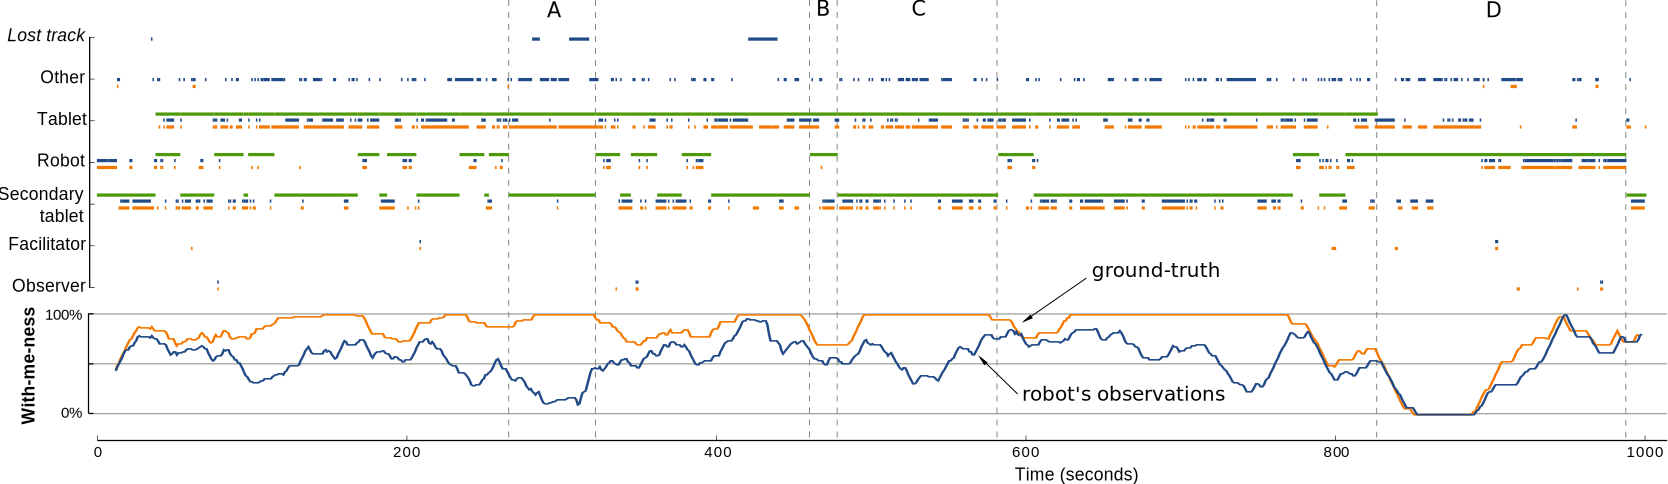
\includegraphics[width=\linewidth]{with-me-ness}
    \caption{\small \textbf{With-me-ness}. Evolution of the level of
        \emph{with-me-ness} over the whole $\approx$20min long interaction of
        subject 4. \emph{Interaction Episodes} describe the distinct phases of
        the interaction, and are discussed in the text. The central chart is
        similar to Figure~\ref{fig:realExpected} with the \emph{expected}
        attentional targets added in green. The bottom diagram represents the
        levels of with-me-ness over successive windows of 30 seconds. The blue
        line is with-me-ness as estimated by the robot, the orange line is
        with-me-ness computed from manually annotated attentional targets. The
        ``holes'' in the with-me-ness computed by the robot correspond to period of time
        where the child's face is not detected.}

    \label{fig:with-me-ness}
\end{figure*}


\begin{table}[h!]
    \centering
    \caption{\textbf{Levels of with-me-ness}. For each subject, the with-me-ness
    level is reported over the whole interaction, either based on the
    ground-truth (\ie \emph{ground-truth with-me-ness}), or based on the focus of
    attention measured by the robot. $\mathcal{W}_{robot}$ is strongly correlated to
    $\mathcal{W}_{groundtruth}$: Pearson's $r(4)=0.50$.}

    \begin{tabular}{p{1cm}cccccccc}
        \toprule
        Subject & 1 & 2 & 3 & 4 & 5 & 6 & {\bf M} & {\it SD} \\
        \midrule
        $\mathcal{W}_{g.truth}$ & 79.3 & 82.6  & 90.5 & 87.9 & 90.7 & 83.6 & {\bf 85.8} & {\it 4.6} \\ 
        $\mathcal{W}_{robot}$ & 52.5 & 55.5 & 74.1 & 52.6 & 60.0 & 66.4 & {\bf 60.2} & {\it 8.6} \\
        \bottomrule
    \end{tabular}
    \label{tab:results-with-me-ness}
\end{table}

Figure~\ref{fig:with-me-ness} can be further analyzed:\fixme{This paragraph
needs to be adapted}
The matching curve (cyan color) shows the overlapping between the
expected and the real focuses of attention. As can be noticed there is a
fluctuation at the beginning of the interaction as well as just before the
activity switching. These chaotic gaze manifestation is what we call an
automatic discovery of events, when the user experiences an uncertainty in the
present situation. 

The first one of the previous two situations presented above is due to the
novelty effect the subjects experience for the first time in front of the system
and according to the rest of participants suggests that the adaptation time is
around the first 2 minutes of interaction. In the second case, an unexpected
robot behavior produces such reaction due to an activity switching, the story
telling.

It is important to consider that in some occasions during the interaction, none
of the focuses of attention were within the field of view due to the time
transition from one focus to another resulting in an ambiguity. In order to deal
with these few cases it is assumed that the minimum distance between the height
of the field of view (cone) and the targets corresponds to the most likely focus
of attention. However, we also want to distinguish such cases when the subject
is directly not looking where the defined targets are located, but towards a
region far from the interaction field. These cases are not common but they can
be easily identified by setting a horizontal threshold to the field of view.

A relevant trend that can be observed is the continuous `look for approval'
situation where the subjects look at the experimenter in order to provide
feedback about the robot's response before providing their own one (see yellow
boxes in figure \ref{fig:realExpected}). Such transition tablet-experimenter
becomes more frequent in several cases, for instance when the experimenter makes
a suggestion (orange box in figure \ref{fig:realExpected}), in this case, switch
to a more complicated word.

Once the turn-taking is established, a pattern becomes visible during the
subject's feedback, when an attempt is performed: Such pattern shows a high
intermittent gaze frequency from the tablet to the selection. It also reveals
that the subject is using the demonstration model in the selection tablet to
provide a better answer to the robot. In fact, subjects decrease the response
time after each shift as well as the gaze frequency towards the model suggesting
an assimilation over time. Moreover, when a new demonstration is selected for
playing, the same behavior is replicated (see yellow boxes in figure
\ref{fig:realExpected}).


If we consider the case shown in section \ref{sec:fromFaceTo}, evaluating the
subject's progression together with the time on task may be an indicator of
engagement: If the subject answers so quickly with respect to the previous
attempts with a poorer handwriting may be the case she is not engaged anymore.
In such hypothetical case an activity switch can be easily implemented in a
robot architecture. It confirms the findings reported in \cite{anzalone} where
time response to event is proposed to account quality of interaction. 
%
%However, a high amount of gaze shift (figure \ref{fig:gazeR}) towards the
%demonstration provided can reveal that the challenge is too big or no gaze, the
%exactly the opposite. In this case, the robot response can be adapted to the
%situation. Similar, but least relevant results are obtained using the
%correctness (figure \ref{fig:errorR}) of the child's feedback after each
%attempt. 
%
%\begin{figure}
%  \centering
%  \begin{tabular}{@{}c@{}}
%    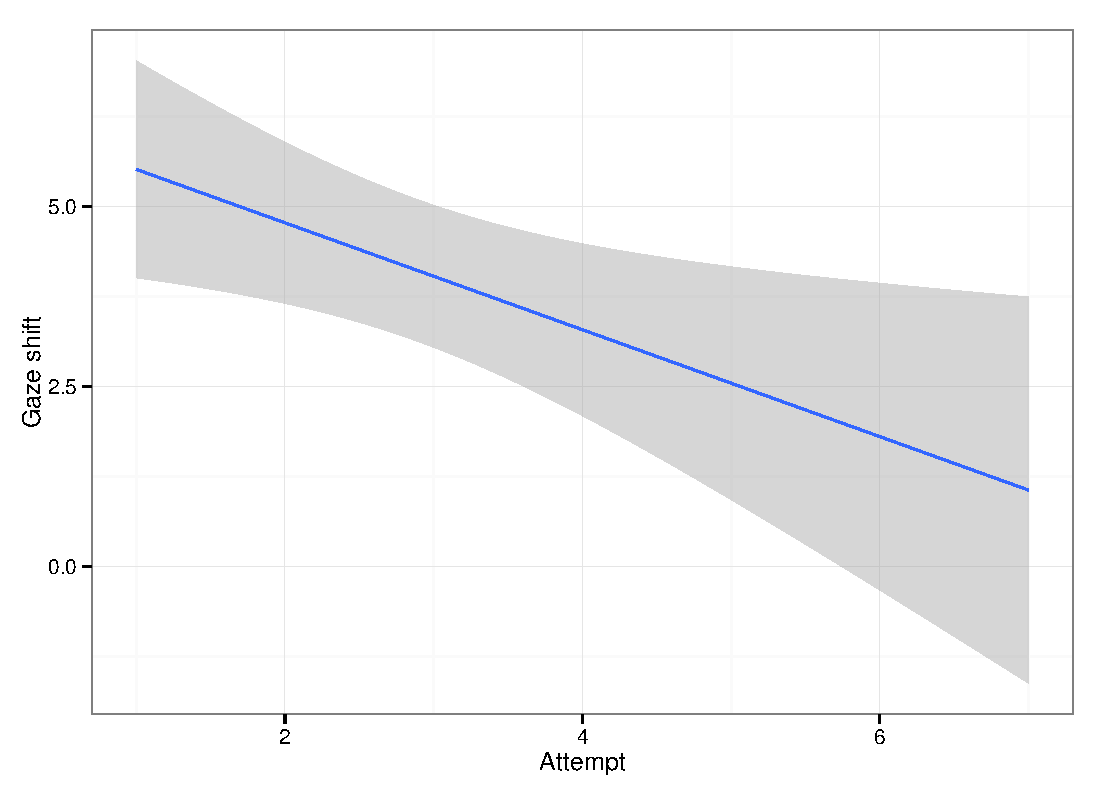
\includegraphics[width=.7\linewidth,height=100pt]{gazeR} \\
%    \small (a) Occurrences of a gaze shift.
%  \end{tabular}\label{fig:gazeR}
%
%  \vspace{\floatsep}
%
%  \begin{tabular}{@{}c@{}}
%    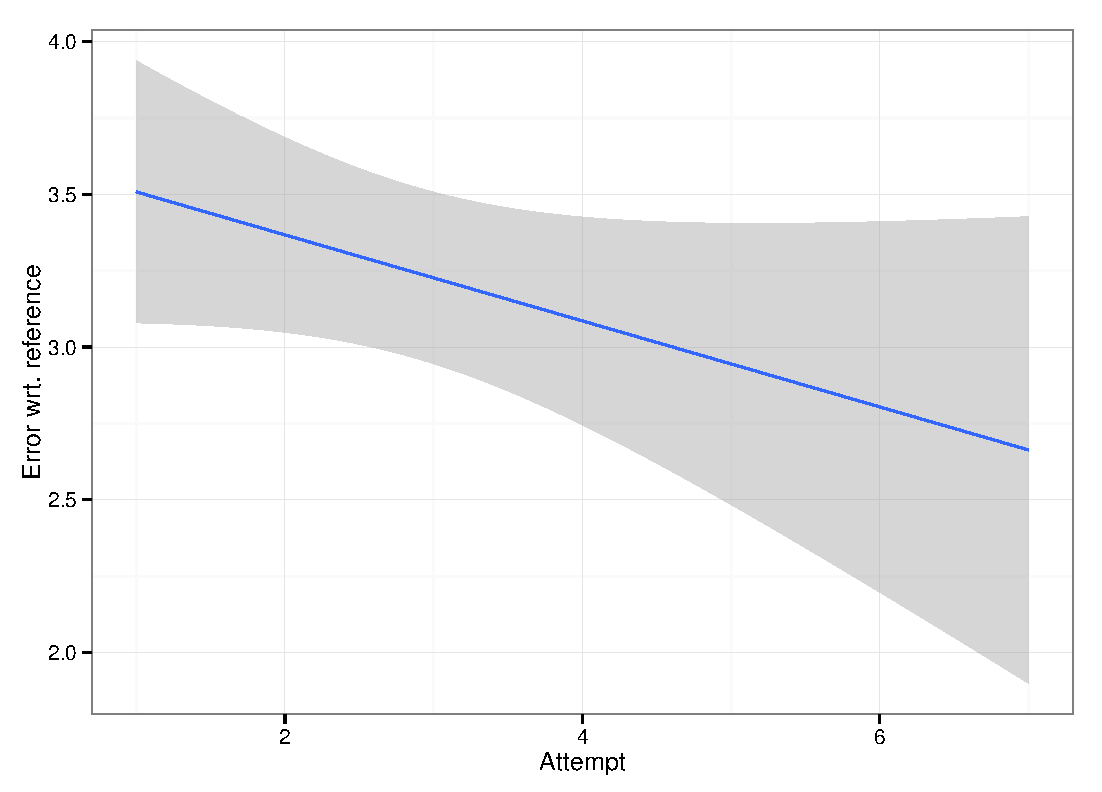
\includegraphics[width=.7\linewidth,height=100pt]{errorR} \\
%    \small (b) Word correctness.
%  \end{tabular}\label{fig:errorR}
%
%  \caption{ \small Linear regression of all subject attempts against the gaze
%  shift tablet-model (a) and the correctness as the average euclidean distance
%  of each letter in its corresponding eigenspace with respect to a reference
%  letter (b). The gray region defines the confidence interval.}
%  
%\end{figure}
%
%
%This information can be used to estimate the child's state during the
%interaction. For instance, if we consider that a low level of engagement is
%produced by extremely high or low demanding situations, it is possible to assess
%the engagement level during the interaction based on gaze shift and word
%correctness.

It is also important to notice that the initiative of the robot into the
learning process in a turn-taking activity produces an effect in the engagement
of the human partner. However, experience suggests that a robot that learns
evoke a positive action in the partner. But the opposite, a robot that is not
able to progress over time, produces the contrary effect.

%Finally, the subjects set their attention more often to the tablet displaying the generated hand-writing during the robot feedback rather than to the robot itself. 

%%%%%%%%%%%%%%%%%%%%%%%%%%%%%%%%%%%%%%%%%%%%%%%%%%%%%%%%%%%%%%%%%%%%%%%%%%%%%%%%%
%%%%%%%%%%%%%%%%%%%%%%%%%%%%%%%%%%%%%%%%%%%%%%%%%%%%%%%%%%%%%%%%%%%%%%%%%%%%%%%%%
%%%%%%%%%%%%%%%%%%%%%%%%%%%%%%%%%%%%%%%%%%%%%%%%%%%%%%%%%%%%%%%%%%%%%%%%%%%%%%%%%


\section{Discussion and Conclusion}

As hinted by the title of this article, we have presented here how a robot can
effectively assess in real-time and with a regular camera the focus of attention
of its interactant, and how we can, in turn, combine it with the robot's {\it a priori}
about the interaction to build a metric of
\emph{with-me-ness} over the course of the interaction.

\paragraph{Head Pose to Assess Attention: is it Relevant?}

%During the case study, results show that it is possible to distinguish between
%long and short feedback episodes based on the gaze shift and depending on the
%previous attempts performed by the subject. As a result, gaze-shift together
%with the number of attempts becomes a reliable indicator candidate in the
%assessment of the engagement during the activity.
%
%Additionally, both the gaze shift and the correctness of the feedback seem to be
%strictly correlated with the learning gain during the activity as they go in
%decrement after each attempt provided by the subjects. Despite the fact that
%these results are encouraging, there is a need of validation with a greater
%amount of subjects.

We already stated the main limitations of our approach to estimation of the
focus of attention: eye gaze information is neglected and we do not perform
actual visibility check of the in focus objects (we simply approximate them to
their origins, ignoring possible occlusions).

While the first issue is shared with most of the other vision (2D or 3D) or motion
capture techniques for real-time gaze estimation found in robotics,
our results are positive: we shows that relying
purely on head pose estimation to estimate gaze direction leads to real-world
measures that are worth being considered and used. They may not match manual
annotations, but they are definitely a valuable \emph{in-the-moment} input for
the robot, reaching for certain children levels of accuracy traditionally
considered as very good.

Interestingly, previous research conducted on ape-human interaction by
Tomasello~\etal~\cite{tomasello2007reliance} shows that apes rely primarily
on the head pose to estimate the focus of attention of a human partner, in to contrast
to human children who primarily rely on eye direction. From this perspective,
our robot mimics attention tracking mechanism comparable to the ones found in apes.

Our approach relies on a simple, non-intrusive sensor (a RGB camera on
the robot) and an open-source, fast pose estimation algorithm\fixme{test on nao!
how fast is it actually?}: we hope that this may contribute to a widespread
adoption of such a technique on a range of robots, including the common {\sc
nao} platform.

%Gaze information acquired during the interactions is not only useful to detect
%and predict engagement, but also allows the possibility to develop actively the
%concept gaze-aware robot. In other words, make the system able to estimate where
%the subject looks at, but also imitate the same subject's VFoA when the activity
%state allows it. 

\paragraph{With-me-ness: yet another metric of engagement?}

Borrowing the neologism from the field of CSCL, we have also introduced in this
article
\emph{with-me-ness} as a measure of ``how much the user in \emph{with} the robot during
a task''. This can be acquired over the course the interaction,
thus providing the robot with a real-time metric for relatively high-level social construct,
undoubtedly related to engagement.

One may reasonably wonder how different is \emph{with-me-ness} from \emph{joint
attention} on one hand, and from \emph{engagement} on the other hand.
With-me-ness is related to both, with however noteworthy nuances: (Triadic) \emph{joint
attention} is understood as the cognitive realization of a shared attention to
an object, itself building on a shared perception of that object (\ie joint attention
builds on a \emph{perceptual} alignment of two agents). \emph{Conceptual
with-me-ness} as proposed by Sharma~\etal is on the contrary \emph{referential}: ``you are
\emph{with} me if you focus on what I refer to, either explicitly or
implicitly''. We propose to understand it here in an even slightly broader sense, that
better reflect the \emph{interaction}: ``you are \emph{with} me if you focus on
what is important for the interactive task at hand.''

On the other hand, with-me-ness is only a precursor of engagement: it
does not say much about the \emph{cognitive} commitment of a user to an interaction. A
user may closely adhere to the injunctions of the robot (or, actually, of the
experimenters), with thus high levels of with-me-ness,  without being \emph{engaged} into the interaction. This is
typically seen in child-robot interaction: children will attempt to closely
follow what they are asked to do -- which may \emph{look like} they are engaged
into the interaction -- while they merely \emph{obey orders}.

Compared to engagement, one of the strength of with-me-ness is its specificity:
it is well-defined, we can formalize it, and
as such, it is valuable to assess and compare how users are willing or able to
interact with a robot. Besides, we have hopefully demonstrated in this article
that with-me-ness is an operational \emph{in-the-moment} metric that can be also
used as feed-back to the robot controller to build richer, more adaptive
interactive behaviors for our robots.

\section*{Acknowledgments}

This research was partially supported by the Funda\c{c}\~{a}o para a Ci\^{e}ncia
e a Tecnologia (FCT) with reference UID/CEC/ 50021/2013, and by the Swiss
National Science Foundation through the National Centre of Competence in
Research Robotics.

\bibliographystyle{abbrv}
\bibliography{sigproc}
\end{document}
